\graphicspath{{./images/chap5/}}
% Sloop-mturk: Crowdsourced relevance feedback on mturk
% Methodology
% * Design and Architecture
% * Population of interest and sampling subject used in the study
% * Instrument and what it measures (metrics)
% * qualifications of informants if used in the study
% * Validation
% * Data gathering procedure (experiments)
\chapter{Crowdsourced Relevance Feedback}
\label{chap:sloop_mturk}
% Sloop-mturk: Crowdsourced relevance feedback on mturk
\section{Sloop MTurk}

As described in \ref{chap:relevance_feedback}, multiple rounds of relevance
feedback accelerates precision and recall of the recognition. This chapter
presents the architecture of \emph{Sloop MTurk}, the crowdsourced relevance
feedback integration of Sloop. 

\begin{figure}[ht]
  \centering
  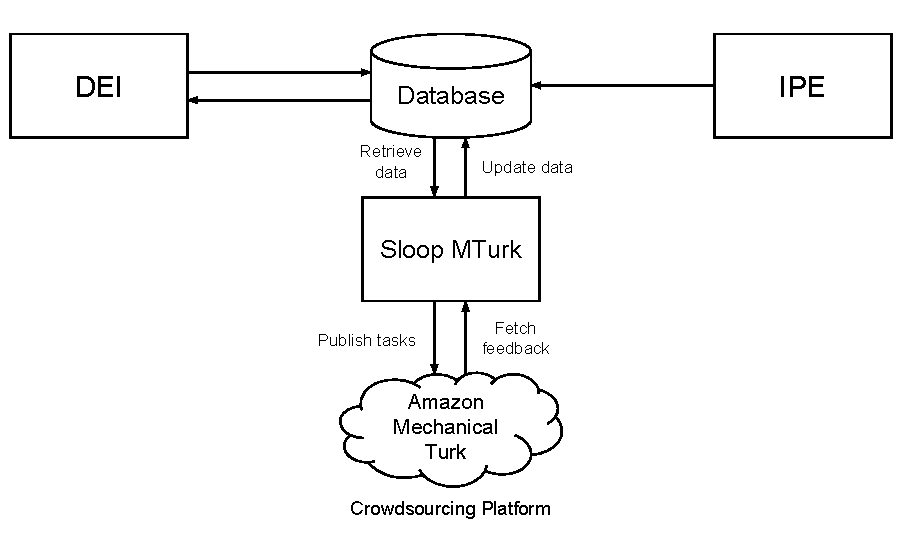
\includegraphics[width=0.8\textwidth]{sloop/turk_system}
  \caption{Sloop Architecture with Sloop MTurk integration}
  \label{fig:turk_overview} %chktex 24
\end{figure}

Sloop MTurk communicates with the crowdsourcing platform in order to provide
human feedback on the original rankings. Our focus is on 

\subsection{Architecture}

Following are the four major functions used within the relevance feedback
workflow.
\begin{enumerate}
	\item Retrieve
	\item Publish
	\item Fetch
	\item Update
\end{enumerate}

\subsubsection{Retrieve}

In the first stage of the relevance feedback workflow, Sloop MTurk retrieves a
number of unknown, and known image pairs from the database in the ratio
described in \ref{subsub:validation}. The metadata about the retrieved pairs,
such as the answers to the known pairs, individual identification numbers, and
source address, is stored in a lightweight SQLite database while the images are
stored separately.

Sloop MTurk never publishes a duplicated \emph{unknown} pair onto MTurk. It
actively checks with the local database before any retrieval if an unknown pair
is ever published before. User can set the sampling policy of Sloop MTurk in
the config file. The default value is set to use the normal sampling on the
median whose performance has been shown in chapter
\ref{chap:relevance_feedback}.

Sloop MTurk only downloads the images necessary for the tasks to minimize the
bandwidth usage. Upon the retrieval, Sloop MTurk caches the image data into its
local storage on the file system running on NGINX. Caching image data on the
filesystem eliminates the network latency and cuts down the data transfer
overhead because fetching large responses, like the images, over the network is
both slow and expensive. The advantage of storing images on the file system,
over storing them in the database, is that we can also refer to the images
hosted on the filesystem in our actual deployment, instead of having to set up
another machine, or to use other external web hosting.

\subsubsection{Publish}

Sloop MTurk publishes the tasks onto MTurk immediately after all the
information is fetched. The tasks published are available on Amazon Mechanical
Turk under the title: 'Image Matching -- Animals' posted by user 'sloop'. 
% TODO Tell user that they need AWS access ID and secret key to programmatically
% communicate with MTurk

\subsubsection{Fetch}

User can fetch the results that are completed via Sloop MTurk fetch. This can
also be set up as a cron job. Sloop MTurk searches for all the reviewable
tasks, and automatically accepts and retrieves the tasks whose answers to all
of the known pairs are correct; otherwise, it rejects the tasks. If a task is
accepted, an amount of payment will be incurred to the user's account to reward
the worker.

Sloop MTurk logs all the answers to the unknown pairs in the accepted
assignments into the local SQLite database. No result are going to be deleted
until the user runs garbage collection command.

\subsubsection{Update}

Update command pushes the answers logged in the local database back to the
original database so that the data is ready for another round of relevance
feedback. The remote database server then infers the captures' cohort from the
data pushed and the existing data, and then performs the merging logic
accordingly\cite{sloopdocs}. 

The update command is separated from fetch for the debugging purpose. In
practice, as we would like to update the upstream database as frequent as
possible as we have seen in the Experiments section in
\ref{chap:relevance_feedback}.

\subsection{Platform Selection}

Workers and requesters interact via a crowdsourcing platform. All of our tasks
are published on Amazon Mechanical Turk (MTurk), which is one of the most
popular crowdsourcing platforms.

\subsection{Human Intelligence Task (HIT)}

Tasks published on MTurk are called Human
Intelligence Tasks (HITs). The term 'HIT' and 'tasks' are going to be used
interchangeably throughout this report.

Requesters publish the tasks that they need to accomplish onto Amazon
Mechanical Turk marketplace with an amount of payment to reward the workers who
finish the tasks.

\subsubsection{Task Design}

A wide variety of tasks can be crowdsourced. There are two possible designs we
have considered:
\begin{itemize}
	\item Rankings and weights
    Each worker may be asked to provide a full rankings or a relative weights
    for a given pool of candidates. Although knowing the correct rankings is
    valuable to ranked retrieval results, which is Sloop preliminary output,
    ultimately, we would like to determine a sharp cutoff between matching
    images and non-matching images so that each individual can be exclusively
    identified. Ranks alone do not provide such cutoff. Even if we knew all the
    correct rankings, we would not be able to decide whether two animals are
    the same individual animals. Thus, rankings and weights is not a viable
    option in this case.
	\item Multiple-choice questions
    A question can include multiple options, for instance, which of the images
    in the choices contains an animal that matches, the given individual
    animal. However, this approach only tells us which of the pictures among
    all the choices best matches a given image, which is an inefficient
    approach of ranking images. Alternatively, we can ask workers to provide
    all the matches among all the options. In this case, there can be none or
    more than one answer. However, using this method, we only gain the
    information of one individual from $n$ comparisons, where $n$ is the number
    of choices for each question.

    We can model our task as a binary questions of whether a pair of images, of
    the same view, contains the same individual animal (Is a match?). Since,
    eventually, all the image pairs will be labelled as either a match or a
    non-match, we will be able to construct a mapping that allows us to
    exclusively identify all the individual animals in the pictures.
\end{itemize}

\subsubsection{Validation}
\label{subsub:validation}

For each task, since the quality of the submitted work is not directly
observable, we add other three \emph{gold standard} questions, for which the
correct answers are known a priori. Among the three questions, one is a known
pair of images containing the same individual, another is a known pair of
images containing different individuals, and the other is a random known pair.
These \emph{gold standard} questions work as qualifying tests for eligible
workers. Additionally, they also accelerate the workers' learning process and
skill level.

To further reassure the correctness of the answers submitted by the workers, we
publish the same assignment to three workers, and estimate the correct answer
by consensus. We only allow workers with task acceptance rate higher than 0.8
to prevent spam. If the majority agrees on some answer, it maybe safe to assume
that it is correct. Obviously, given a task, the more number of workers we
assign, the less chance there is of getting an incorrect answer. However, the
budget and the time it takes to complete all the assignments is going to
increase linearly as we increase the number of the workers, while the
correctness only increases logarithmically. Therefore, we decided to publish
exactly three assignments, which is the minimal number to reach a consensus,
for each task.

\subsection{Cost Model}

Sloop MTurk uses the evaluation metrics mentioned in chapter
\ref{chap:relevance_feedback} to measure the performance of the system.

\subsubsection{Correctness}

To analyze the correctness, we are still using the Mean Average Precision to
evaluate the correctness of the results. MAP has been shown to have especially
good discrimination and stability on evaluating information retrieval
systems\cite{manning2008introduction}.

\subsubsection{Expense}

Each worker, upon completion of a task, receives the posted price for that
task. The more tasks published, the higher the total payment we have to make.

In the actual production of Sloop, the inconsistence results from such error is
detectable and will be submitted for manual review. The conflicts are going to
be resolve by the biologists or relevant expert, whose time and effort is a
relatively more valuable than that of the online workers. In this case, the
cost incurred by the manual review is going to be higher than the cost of the
payment we need to reward the workers. Quantitatively, for each manual review,
the cost is going to be the number of all the captures involved in the conflict
multiplied by a constant.
